\section{Exercises}

%%%%%%%%%%%%%%%%%%%%%

\subsection{Introduction to multiple regression}

% 1 

\eoce{In Chapter 6 you were introduced to a data set from an experiment to measure and compare the effectiveness of various feed supplements on the growth rate of chickens. Newly hatched chicks were randomly allocated into six groups, and each group was given a different feed supplement. Their weights in grams after six weeks are given along with feed types in the data set called \texttt{chickwts}. We are specifically interested in the effect of casein feed on the weights of these chicks, so we have created a variable called \texttt{casein} and coded chicks who were on casein feed as 1 and those who were on other diets as 0. The summary table below shows the results of a simple linear regression model for predicting \texttt{weight} from \texttt{casein}. \citep{data:chickwts}
\begin{center}
\begin{tabular}{r r r r r}
  \hline
 & Estimate & Std. Error & t value & Pr($>$$|$t$|$) \\ 
  \hline
(Intercept) & 248.64 & 9.54 & 26.06 & 0.0000 \\ 
  casein & 74.94 & 23.21 & 3.23 & 0.0019 \\ 
   \hline
\end{tabular}
\end{center}
\begin{enumerate}[(a)]
\setlength{\itemsep}{0mm}
\item Write the equation of the regression line.
\item Interpret the slope in context, and calculate the predicted weight of chicks who are and who not are on another feed.
\item Is there a statistically significant relationship between feed type (casein or other) and the average weight of chicks? State the hypotheses and include any information used to conduct the test. Note that if we look back at Exercise~\ref{chickwts} on page~\pageref{chickwts}, we would see that the variability within the casein group and the variability across the other groups are about equal and the distributions symmetric. With these conditions satisfied, it is reasonable to proceed with the test. (Note also that we don't need to check linearity since the predictor has only two levels.)
\end{enumerate}
}
{
\begin{enumerate}[(a)]
\setlength{\itemsep}{0mm}
\item $\widehat{weight} = 248.64 + 74.94 \times casein$
\item The estimated mean weight of chicks who are on casein feed is 74.94 grams higher than those who are given other feeds. \\
Casein: $\widehat{weight} = 248.64 + 74.94 \times 1 = 323.58$ grams \\
No casein: $\widehat{weight} = 248.64 + 74.94 \times 0 = 248.64$ grams
\item $H_0$: The true coefficient for \texttt{casein} is zero ($\beta_1 = 0$). \\
$H_A$: The true coefficient for \texttt{casein} is not zero ($\beta_1 \ne 0$). \\
The question is asking whether any relationship exists
 between feed type and weight, therefore we use a two-sided alternative hypothesis. $T = 3.23$, and the p-value is approximately 0.0019. With such a low p-value, we reject $H_0$. The data provide convincing evidence that the true slope parameter is different than 0, and hence there appears to be a statistically significant relationship between feed type (casein or other) and the average weight of chicks. 
\end{enumerate}
}\label{chickwtsCasein}

% 2

\eoce{Vitamin C is believed to help promote dental health. One common way to get Vitamin C is by drinking orange juice. Another option is to take ascorbic acid tablets. An experiment was conducted to test if one source is more effective than the other. 60 guinea pigs were randomly assigned to these two delivery methods for Vitamin C, 30 in each group. The length of teeth in millimeters are given along with delivery methods in the data set called \texttt{ToothGrowth}. We created a variable called \texttt{OJ} and coded guinea pigs who were given orange juice as 1 and those who were given ascorbic acid as 0. The summary table below shows the results of a simple linear regression model for predicting the average tooth length, \texttt{len}, from \texttt{OJ}. \citep{data:ToothGrowth}
\begin{center}
\begin{tabular}{rrrrr}
  \hline
 & Estimate & Std. Error & t value & Pr($>$$|$t$|$) \\ 
  \hline
(Intercept) & 16.96 & 1.37 & 12.42 & 0.0000 \\ 
  oj & 3.70 & 1.93 & 1.92 & 0.0604 \\ 
   \hline
\end{tabular}
\end{center}
\begin{enumerate}[(a)]
\setlength{\itemsep}{0mm}
\item Write the equation of the regression line.
\item Interpret the slope in context, and calculate the predicted tooth length for guinea pigs who were given orange juice and those who were given ascorbic acid.
\item Is there a statistically significant relationship between the average tooth length and delivery method of Vitamin C in guinea pigs? State the hypotheses and include any information used to conduct the test. Note that the variability within the orange juice and the ascorbic acid groups are about equal and the distributions symmetric. With these conditions satisfied, it is reasonable to proceed with the test.
\end{enumerate}
}
{
\begin{enumerate}[(a)]
\setlength{\itemsep}{0mm}
\item $\widehat{length} = 16.96 + 1.93 \times oj$
\item The estimated mean tooth length of guinea pigs who are given orange juice is 1.93 millimeters longer than those who are given ascorbic acid. \\
Orange juice: $\widehat{length} = 16.96 + 1.93 \times 1 = 18.89~millimeters $ \\
Ascorbic acid: $\widehat{length} = 16.96 + 1.93 \times 0 = 16.96~millimeters $ 
\item $H_0$: The true coefficient for \texttt{oj} is zero ($\beta_1 = 0$). \\
$H_A$: The true coefficient for \texttt{oj} is not zero ($\beta_1 \ne 0$). \\
The question is asking whether any relationship exists
 between tooth length and delivery method of Vitamin C, therefore we use a two-sided alternative hypothesis. $T = 1.92$, and the p-value is approximately 0.0604. If using a 5\% significance level, since p-value $>$ 0.05, we fail to reject $H_0$. The data do not provide convincing evidence that the true slope parameter is different than 0, and hence there does not appear to be a statistically significant relationship between the average tooth length and delivery method of Vitamin C in guinea pigs.
\end{enumerate}
}

% 3

\eoce{The Child Health and Development Studies (CHDS) is a collection of studies, one of which considers all pregnancies between 1960 and 1967 among women in the Kaiser Foundation Health Plan in the San Francisco East Bay area. A random sample of these data are given in a data set called \texttt{babies}. We consider the relationship between smoking and weight of the baby. The variable \texttt{smoke} is coded 1 if the mother is a smoker, and 0 if not. The summary table below shows the results of a simple linear regression model for predicting the average birth weight of babies, measured in ounces (\texttt{bwt}), from \texttt{smoke}. \citep{data:babies}
\begin{center}
\begin{tabular}{rrrrr}
  \hline
 & Estimate & Std. Error & t value & Pr($>$$|$t$|$) \\ 
  \hline
(Intercept) & 123.05 & 0.65 & 189.60 & 0.0000 \\ 
  smoke & -8.94 & 1.03 & -8.65 & 0.0000 \\ 
   \hline
\end{tabular}
\end{center}
The variability within the smokers and non-smokers are about equal and the distributions symmetric. With these conditions satisfied, it is reasonable to proceed with the test. (Note that we don't need to check linearity since the predictor has only two levels.)
\begin{enumerate}[(a)]
\setlength{\itemsep}{0mm}
\item Write the equation of the regression line.
\item Interpret the slope in context, and
 calculate the predicted birth weight of babies born to smoker and non-smoker mothers.
\item Is there a statistically significant relationship between the average birth weight and smoking? State the hypotheses and include any information used to conduct the test.
\end{enumerate}
}
{
\begin{enumerate}[(a)]
\setlength{\itemsep}{0mm}
\item $\widehat{bwt} = 123.05 - 8.94 \times smoke$
\item The estimated body weight of babies born to smoking mothers is 8.94 ounces lower than those who are born to non-smoking mothers. \\
Smoker: $\widehat{bwt} = 123.05 - 8.94 \times 1 = 114.11$ ounces \\
Non-smoker: $\widehat{bwt} = 123.05 - 8.94 \times 0 = 123.05$ ounces
\item $H_0$: The true coefficient for \texttt{smoke} is zero ($\beta_1 = 0$). \\
$H_A$: The true coefficient for \texttt{smoke} is not zero ($\beta_1 \ne 0$). \\
The question is asking whether any relationship exists between smoking and birth weight, therefore we use a two-sided alternative hypothesis. $T= -8.65$, and the p-value is approximately 0. Since p-value is very small we reject $H_0$. The data provide convincing evidence that the true slope parameter is different than 0 and that the linear relationship between birth weight and smoking is real.
\end{enumerate}
}\label{babiesWeight}

% 4

\eoce{Exercise~\eoceref{babiesWeight} introduces a data set on birth weight of babies. Another variable we consider is \texttt{parity}, where 0 is first born, and 1 is otherwise. The summary table below shows the results of a simple linear regression model for predicting the average birth weight of babies, measured in ounces, from \texttt{parity}. 
\begin{center}
\begin{tabular}{rrrrr}
  \hline
 & Estimate & Std. Error & t value & Pr($>$$|$t$|$) \\ 
  \hline
(Intercept) & 120.07 & 0.60 & 199.94 & 0.0000 \\ 
  parity & -1.93 & 1.19 & -1.62 & 0.1052 \\ 
   \hline
\end{tabular}
\end{center}
\begin{enumerate}[(a)]
\setlength{\itemsep}{0mm}
\item Write the equation of the regression line.
\item Interpret the slope in context, and calculate the predicted birth weight of first borns and others.
\item Is there a statistically significant relationship between the average birth weight and parity? State the hypotheses and include any information used to conduct the test.
\end{enumerate}
}
{
\begin{enumerate}[(a)]
\setlength{\itemsep}{0mm}
\item $\widehat{bwt} = 120.07 - 1.93 \times parity $
\item The estimated body weight of first borns is 1.93 ounces lower than others. \\
Smoker: $\widehat{bwt} = 120.07 - 1.93 \times 1 = 118.14~ounces $ \\
Non-smoker: $\widehat{bwt} = 120.07 - 1.93 \times 0 = 120.07 ~ounces $ 
\item $H_0$: The true coefficient for \texttt{parity} is zero ($\beta_1 = 0$). \\
$H_A$: The true coefficient for \texttt{parity} is not zero ($\beta_1 \ne 0$). \\
The question is asking whether any relationship exists
 between parity and birth weight, therefore we use a two-sided alternative hypothesis. $T = -1.62$, and the p-value is approximately 0.1052. If using a 5\% significance level, since p-value $>$ 0.05, we fail to reject $H_0$. The data do not provide convincing evidence that the true slope parameter is different than 0, and hence there does not appear to be a statistically significant relationship between birth weight and parity.
\end{enumerate}
}\label{babiesParity}

\pagebreak
% 5

\eoce{The \texttt{babies} dataset used in Exercises \eoceref{babiesWeight} and \eoceref{babiesParity} includes information on length of pregnancy in days (\texttt{gestation}), mother's age in years (\texttt{age}), mother's height in inches (\texttt{height}), and mother's pregnancy weight in pounds (\texttt{weight}), in addition to the \texttt{smoking} and \texttt{parity} variables considered earlier. Below are three observations from this data set. 
\begin{center}
\begin{tabular}{r c c c c c c c}
  \hline
 & bwt & gestation & parity & age & height & weight & smoke \\ 
  \hline
1 & 120 & 284 &   0 &  27 &  62 & 100 &   0 \\ 
  2 & 113 & 282 &   0 &  33 &  64 & 135 &   0 \\ 
$\vdots$ & $\vdots$ & $\vdots$ &   $\vdots$ &  $\vdots$ &  $\vdots$ & $\vdots$ &   $\vdots$ \\ 
  1236 & 117 & 297 &   0 &  38 &  65 & 129 &   0 \\ 
   \hline
\end{tabular}
\end{center}
The summary table below shows the results of a linear regression model for predicting the average birth weight of babies based on all of the variables included in the data set.
\begin{center}
\begin{tabular}{rrrrr}
  \hline
 & Estimate & Std. Error & t value & Pr($>$$|$t$|$) \\ 
  \hline
(Intercept) & -80.41 & 14.35 & -5.60 & 0.0000 \\ 
  gestation & 0.44 & 0.03 & 15.26 & 0.0000 \\ 
  parity & -3.33 & 1.13 & -2.95 & 0.0033 \\ 
  age & -0.01 & 0.09 & -0.10 & 0.9170 \\ 
  height & 1.15 & 0.21 & 5.63 & 0.0000 \\ 
  weight & 0.05 & 0.03 & 1.99 & 0.0471 \\ 
  smoke & -8.40 & 0.95 & -8.81 & 0.0000 \\ 
   \hline
\end{tabular}
\end{center}
\begin{enumerate}[(a)]
\setlength{\itemsep}{0mm}
\item Write the equation of the regression line that includes all of the variables.
\item Interpret the slopes of \texttt{gestation} and \texttt{age} in context.
\item The coefficient for \texttt{parity} is different than in the simple linear model shown in Exercise~\eoceref{babiesParity}. Why might there be a difference?
\item Calculate the residual for the first observation in the data set.
\end{enumerate}
}
{
\begin{enumerate}[(a)]
\setlength{\itemsep}{0mm}
\item $\widehat{bwt} = -80.41 + 0.44 \times gestation - 3.33 \times parity - 0.01 \times age + 1.15 \times height + 0.05 \times weight - 8.40 \times smoke$.
\item $\beta_1$: The model predicts a 0.44 ounce increase in the birth weight of the baby for each additional day in length of pregnancy, all else held constant. \\
$\beta_3$: The model predicts a 0.01 ounce decrease in the birth weight of the baby for each additional year in mother's age, all else held constant. 
\item Parity might be correlated with one of the other variables in the model, which introduces collinearity and complicates model estimation.
\item $\widehat{bwt} = -80.41 + 0.44 \times 284 - 3.33 \times 0 - 0.01 \times 27 + 1.15 \times 62 + 0.05 \times 100 - 8.40 \times 0 = 120.58$ \\
$e = bwt - \widehat{bwt} = 120 - 120.58 = -0.58$
\end{enumerate}
}\label{babiesMR}

% 6

\eoce{Researchers interested in the relationship between absenteeism from school and certain demographic characteristics of children collected data from 146 randomly sampled students in rural New South Wales in a particular school year. These data are given in a data set called \texttt{quine}. Below are three observations from this data set. 
\begin{center}
\begin{tabular}{r c c c c}
\hline
 	& eth 	& sex 	& lrn 		& days \\   
\hline
1 	& 0 		& 1 		& 1 		&   2 \\ 
2 	& 0 		& 1 		& 1 		&  11 \\ 
$\vdots$ & $\vdots$ & $\vdots$ &   $\vdots$ &  $\vdots$  \\ 
146 & 1 		& 0 		& 0 		&  37 \\ 
   \hline
\end{tabular}
\end{center}
The summary table below shows the results of a linear regression model for predicting the average number of days absent based on ethnic background (\texttt{eth}: 0 - aboriginal, 1 - not aboriginal), sex (\texttt{sex}: 0 - female, 1 - male), and learner status (\texttt{lrn}: 0 - average learner, 1 - slow learner). \citep{data:quine}
\begin{center}
\begin{tabular}{rrrrr}
  \hline
 & Estimate & Std. Error & t value & Pr($>$$|$t$|$) \\ 
  \hline
(Intercept) & 18.93 & 2.57 & 7.37 & 0.0000 \\ 
  eth & -9.11 & 2.60 & -3.51 & 0.0000 \\ 
  sex & 3.10 & 2.64 & 1.18 & 0.2411 \\ 
  lrn & 2.15 & 2.65 & 0.81 & 0.4177 \\ 
   \hline
\end{tabular}
\end{center}
\begin{enumerate}[(a)]
\setlength{\itemsep}{0mm}
\item Write the equation of the regression line.
\item Interpret each one of the slopes in context.
\item Calculate the residual for the first observation in the data set.
\end{enumerate}
}
{
\begin{enumerate}[(a)]
\setlength{\itemsep}{0mm}
\item $\widehat{days} =  18.93 - 9.11 \times eth + 3.10 \times sex + 2.15 \times lrn$
\item $\beta_1$: The estimated absence days of students who are not aboriginal is 9.11 lower than the aboriginal students. \\
$\beta_2$: The estimated absence days of male students is 3.10 days higher than females. \\
$\beta_3$: The estimated absence days of students who are slow learners is 2.15 days higher than students who are average learners.
\item $\widehat{days} =  18.93 -9 .11 \times 0 + 3.10 \times 1 + 2.15 \times 1 = 24.18$ \\
$e = days - \widehat{days} = 2 - 24.18 = -22.18$
\end{enumerate}
}\label{daysAbsent}

% 7

\eoce{The variance of the residuals for the model given in Exercise~\eoceref{babiesMR} is 249.28, and the variance of the birth weights of all babies in the data set is 332.57. Calculate the $R^2$ and the adjusted $R^2$. Note that there are 1236 observations in the data set.}
{
The $R^2$ and the adjusted $R^2$ can be calculated as follows:
\begin{align*}
R^2 &= 1 - \frac{Var(e_i)}{Var(y_i)} = 1 - \frac{249.28}{332.57} = 0.2504 \\
R_{adj}^2 &= 1 - \frac{Var(e_i) / (n - p - 1)}{Var(y_i) / (n - 1)} = 1 - \frac{249.28 / (1236 - 6 - 1)}{332.57 / (1236 - 1)} = 0.2468 \\
\end{align*}
}

% 8

\eoce{The variance of the residuals for the model given in Exercise~\eoceref{daysAbsent} is 240.57, and the variance of the number of absent days for all students in the data set is 264.17. Calculate the $R^2$ and the adjusted $R^2$. Note that there are 146 observations in the data set.}
{
The $R^2$ and the adjusted $R^2$ can be calculated as follows:
\begin{align*}
R^2 &= 1 - \frac{Var(e_i)}{Var(y_i)} = 1 - \frac{240.57}{264.17} = 0.0893 \\
R_{adj}^2 &= 1 - \frac{Var(e_i) / (n - p - 1)}{Var(y_i) / (n - 1)} = 1 - \frac{240.57 / (146 - 3 - 1)}{264.17 / ( 146 - 1)} = 0.0701 \\
\end{align*}
}

%%%%%%%%%%%%%%%%%%%%%

\subsection{Model selection}

%%%%%%%%%%%%%%%%%%%%%

% 9

\eoce{Exercise~\eoceref{babiesMR} presents summary output for a regression model for predicting the average birth weight of babies based on six explanatory variables. 
\begin{enumerate}[(a)]
\setlength{\itemsep}{0mm}
\item Determine which variable(s) do not have a significant relationship with the outcome and should be candidates for removal from the model. If there is more than one such model, indicate which one should be removed first.
\item The summary table below shows the results of the regression we refit after removing \texttt{age} from the model. Determine if any other variable(s) should be removed from the model.
\begin{center}
\begin{tabular}{rrrrr}
  \hline
 & Estimate & Std. Error & t value & Pr($>$$|$t$|$) \\ 
  \hline
(Intercept) & -80.64 & 14.04 & -5.74 & 0.0000 \\ 
  gestation & 0.44 & 0.03 & 15.28 & 0.0000 \\ 
  parity & -3.29 & 1.06 & -3.10 & 0.0020 \\ 
  height & 1.15 & 0.20 & 5.64 & 0.0000 \\ 
  weight & 0.05 & 0.03 & 2.00 & 0.0459 \\ 
  smoke & -8.38 & 0.95 & -8.82 & 0.0000 \\ 
   \hline
\end{tabular}
\end{center}
\end{enumerate}
}
{
\begin{enumerate}[(a)]
\setlength{\itemsep}{0mm}
\item There does not appear to be a significant relationship between the age of the mother and the birth weight of the baby since the p-value for the \texttt{age} variable is relatively high. We might consider removing this variable from the model.
\item No, all variables in the model now appear to have a significant relationship with the outcome therefore we would not need to removed any more variables.
\end{enumerate}
}\label{babiesMRfinal}

% 10

\eoce{Exercise~\eoceref{daysAbsent} presents summary output for a regression model for predicting the average number of days absent based on three explanatory variables.
 \begin{enumerate}[(a)]
\setlength{\itemsep}{0mm}
\item Determine which variable(s) do not have a significant relationship with the outcome and should be candidates for removal from the model. If there is more than one such model, indicate which one should be removed first.
\item The summary table below shows the results of the regression we refit after removing learner status from the model. Determine if any other variable(s) should be removed from the model.
\begin{center}
\begin{tabular}{rrrrr}
  \hline
 & Estimate & Std. Error & t value & Pr($>$$|$t$|$) \\ 
  \hline
(Intercept) & 19.98 & 2.22 & 9.01 & 0.0000 \\ 
  eth & -9.06 & 2.60 & -3.49 & 0.0006 \\ 
  sex & 2.78 & 2.60 & 1.07 & 0.2878 \\ 
   \hline
\end{tabular}
\end{center}
\end{enumerate}
}
{
\begin{enumerate}[(a)]
\setlength{\itemsep}{0mm}
\item There does not appear to be a significant relationship between sex and the learner status of the student and number of days absent from school since the p-values for both of these variables is high. We would first consider removing leaner status from the model since the p-value for \texttt{lrn} is higher than the p-value for \texttt{sex}.
\item Yes, next we would consider removing \texttt{sex} from the model since the p-value for this variable is still high.
\end{enumerate}
}

\pagebreak
% 11

\eoce{Exercise~\eoceref{babiesMR} provides regression output for the full model (including all explanatory variables available in the data set) for predicting birth weight of babies. In this exercise, we consider a forward-selection algorithm and add variables to the model one-at-a-time. The table below shows the p-value and adjusted $R^2$ of each model where we include only the corresponding predictor. Based on this table, which variable should be added to the model first?
\begin{center}
\begin{tabular}{l c c c c c c}
\hline
variable		& gestation			& parity	& age	& height 				& weight 				& smoke \\
\hline
p-value		& $2.2 \times 10^{-16}$	& 0.1052	& 0.2375	& $2.97 \times 10^{-12}$	& $8.2 \times 10^{-8}$	& $2.2 \times 10^{-16}$ \\
$R_{adj}^2$	& 0.1657				& 0.0013	& 0.0003	& 0.0386				& 0.0229				& 0.0569 \\
\hline
\end{tabular}
\end{center}
}
{
Based on the p-value alone, either gestation or smoke should be added to the model first. However, since the adjusted $R^2$ for the model with gestation is higher, it would be preferable to add gestation in the first step of the forward-selection algorithm. (Other explanations are possible. For instance, it would be reasonable to only use the adjusted $R^2$.)
}

% 12

\eoce{Exercise~\eoceref{daysAbsent} provides regression output for the full model (including all explanatory variables available in the data set) for predicting number of days absent from school. In this exercise, we consider a forward-selection algorithm and add variables to the model one-at-a-time. The table below shows the p-value and adjusted $R^2$ of each model where we include only the corresponding predictor. Based on this table, which variable should be added to the model first?
\begin{center}
\begin{tabular}{l c c c}
\hline
variable		& ethnicity		& sex	& leaner status	 \\
\hline
p-value		& 0.0007		& 0.3142	& 0.5870	 \\
$R_{adj}^2$	& 0.0714		& 0.0001	& 0 \\
\hline
\end{tabular}
\end{center}
}
{
The first variable to be added to the model is ethnicity.
}

%%%%%%%%%%%%%%%%%%%%%

\subsection{Checking model assumptions using graphs}

%%%%%%%%%%%%%%%%%%%%%

% 13

\eoce{Exercise~\eoceref{babiesMRfinal} presents a regression model for predicting the average birth weight of babies based on length of gestation, parity, height, weight, and smoke. Determine if the model assumptions are met using the plots below. If not, describe how to proceed with the analysis.
\begin{center}
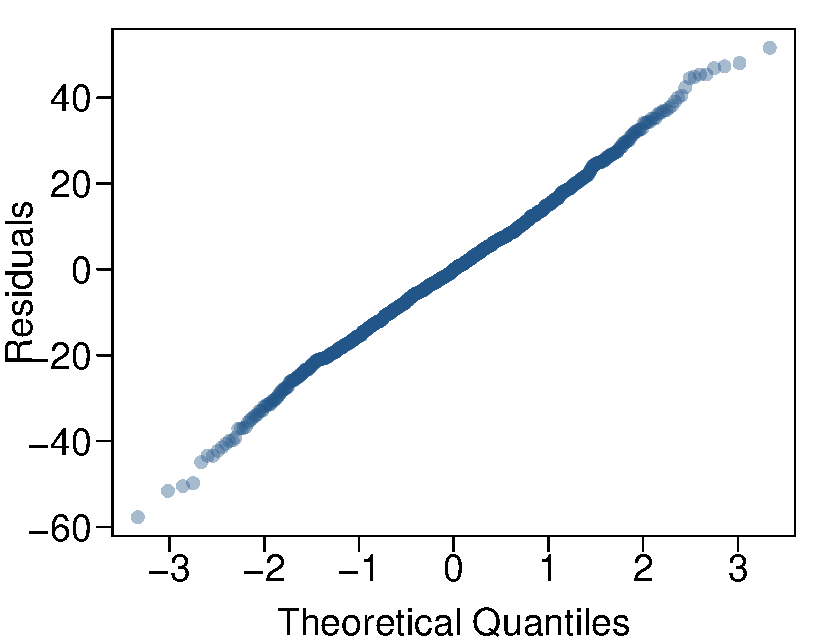
\includegraphics[width=0.425\textwidth]{08/figures/eoce/lmBabies2normProbRes} 
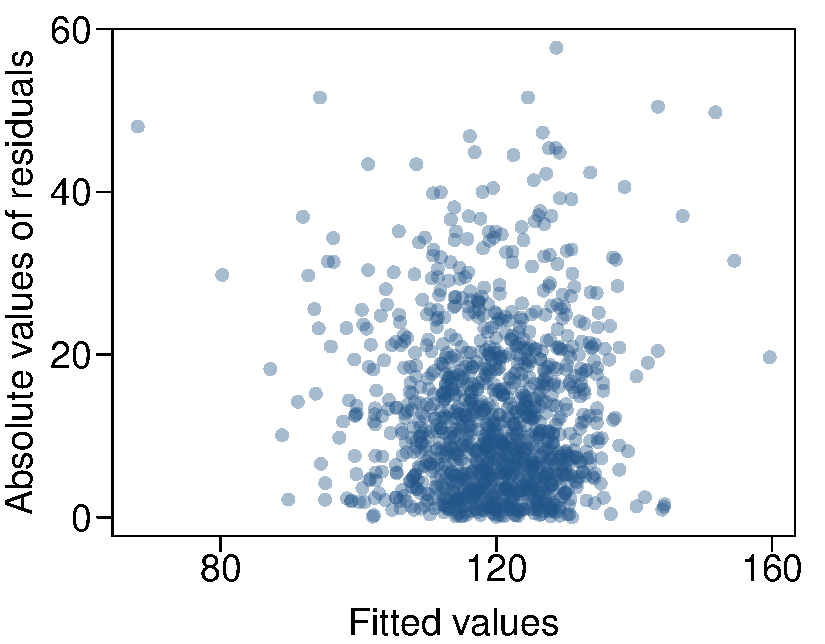
\includegraphics[width=0.425\textwidth]{08/figures/eoce/lmBabies2absResFit} \\
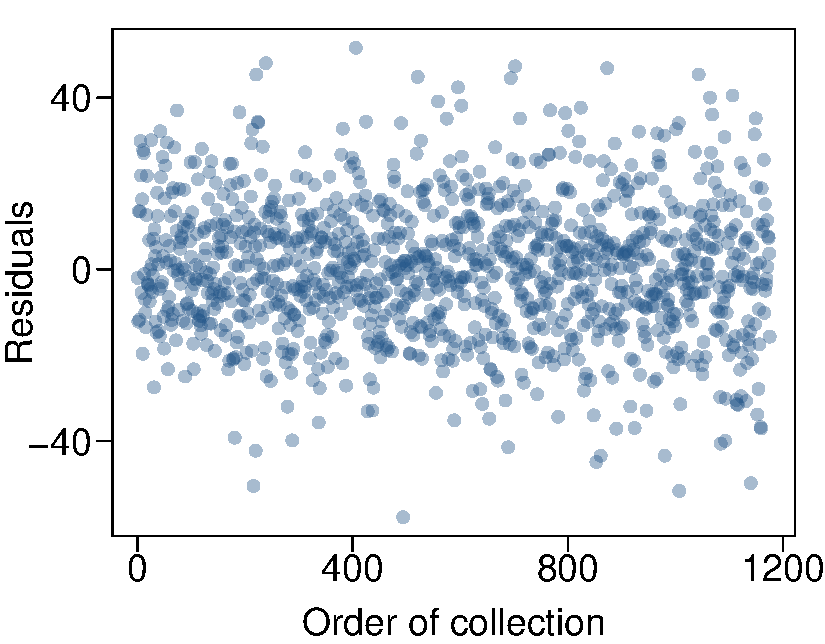
\includegraphics[width=0.425\textwidth]{08/figures/eoce/lmBabies2resOrder}
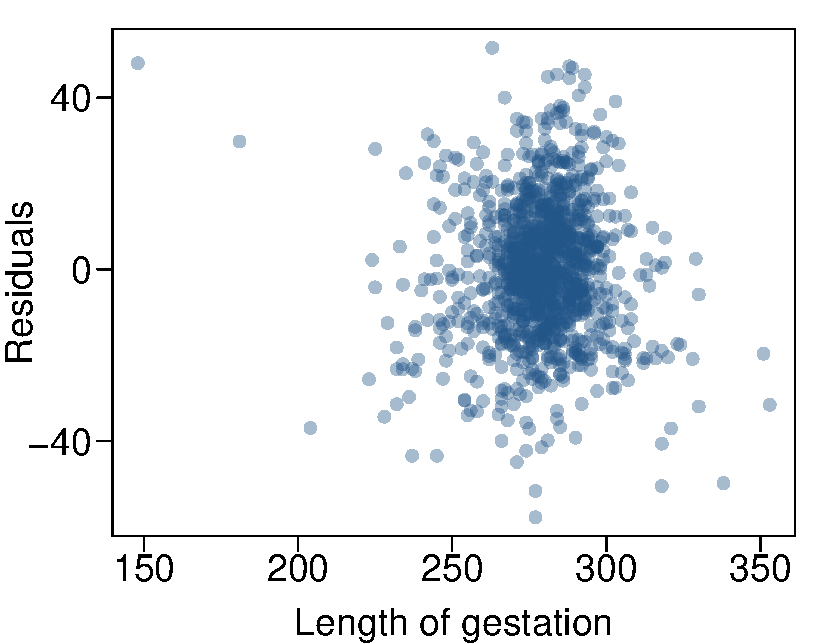
\includegraphics[width=0.425\textwidth]{08/figures/eoce/lmBabies2resGest}  \\ 
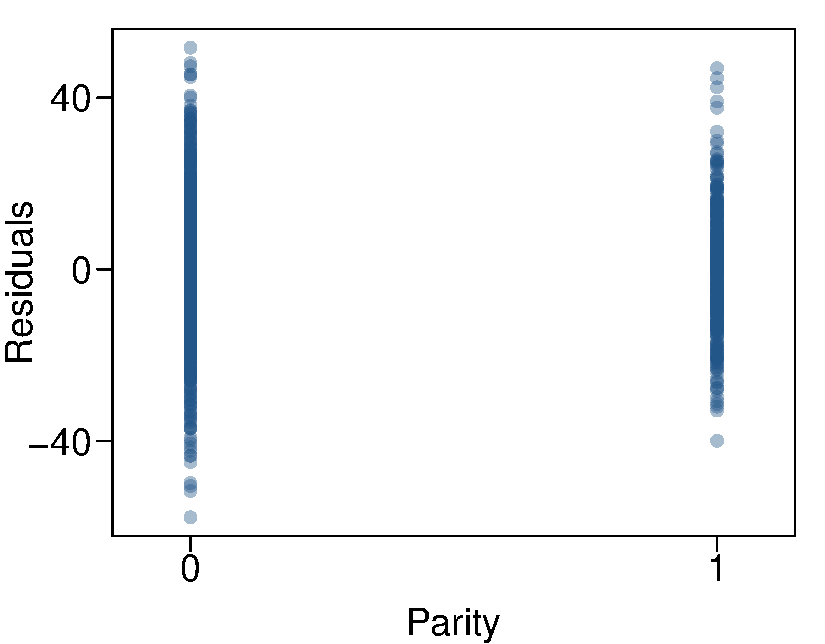
\includegraphics[width=0.4\textwidth]{08/figures/eoce/lmBabies2resParity} 
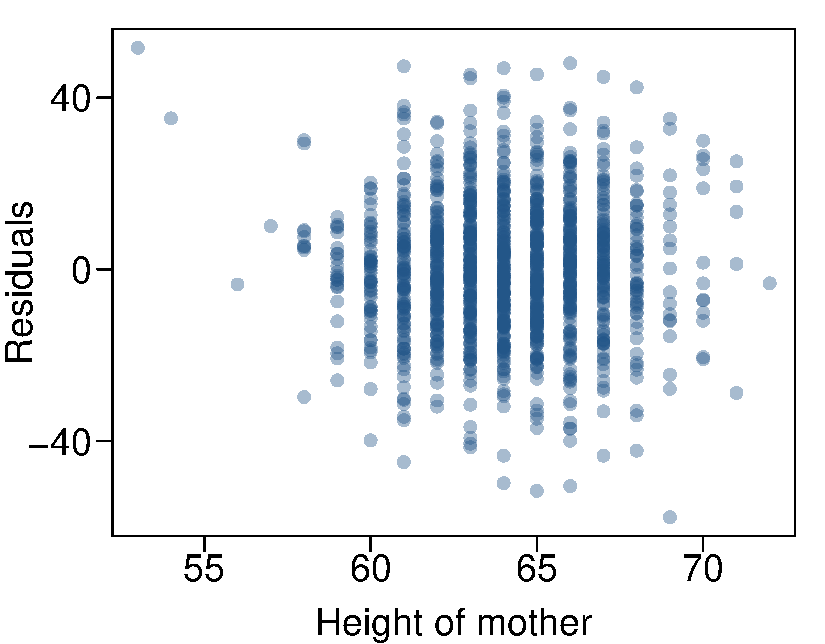
\includegraphics[width=0.4\textwidth]{08/figures/eoce/lmBabies2resHgt} \\
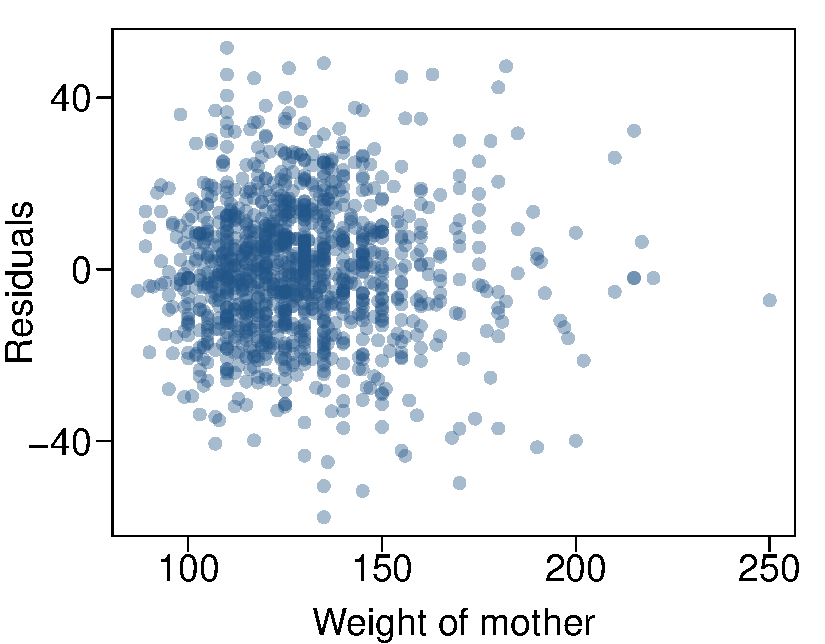
\includegraphics[width=0.4\textwidth]{08/figures/eoce/lmBabies2resWgt} 
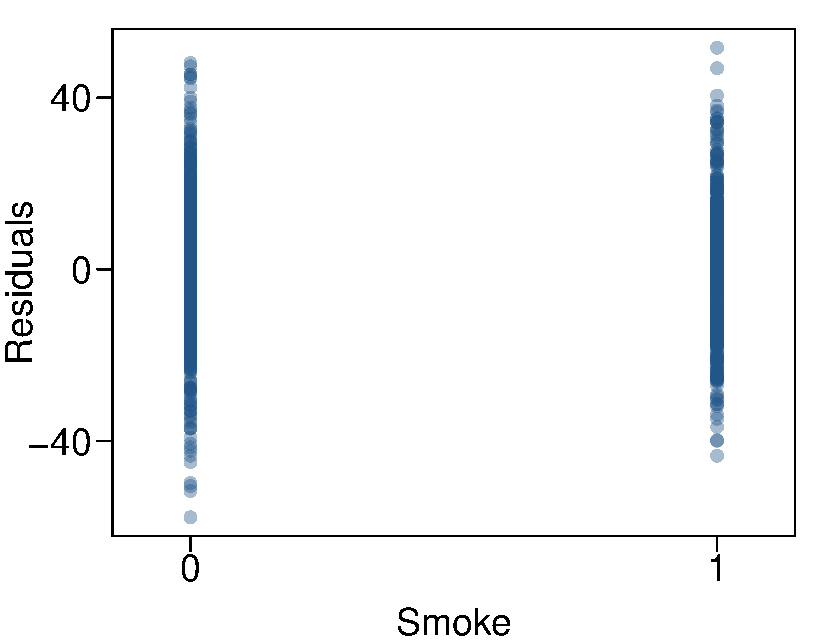
\includegraphics[width=0.4\textwidth]{08/figures/eoce/lmBabies2resSmoke} 
\end{center}
}
{
Listed below are four assumptions that should be satisfied for a multiple regression model to be appropriate, and an analysis of whether or not these are met:
\begin{enumerate}[1.]
\item The residuals of the model should be nearly normal: The normal probability plot shows a nearly normal distribution of the residuals, however, there are some minor irregularities at the tails indicating potential outliers.
\item The variability of the residuals should be nearly constant: The scatterplot of the absolute values of residuals versus the fitted values suggests that there may be a few outliers, some with lower than average fitted values and some with higher than average fitted values.
\item The residuals should be independent: The scatterplot of residuals versus the order of data collection shows a random scatter suggesting that this assumption is met.
\item Each variable should be linearly related to the outcome: The residuals vs. height and weight of mother are randomly distributed around 0. However the residuals vs. length of gestation plot is a little more difficult to judge due to the two clear outliers with low lengths of gestation. The rest of the residuals do appear to be randomly distributed around 0. In addition, the residuals do appear to have constant variability between the two parity and smoking status groups.
\end{enumerate}
Since some of the assumptions are not met, the regression model may not be appropriate for these data. The next step in the analysis should be investigating the outlying observations.
}

% 14

\eoce{The table below presents summary output for a regression model for predicting the average GPA based IQ and gender, where 0 represents a female and 1 represents a male.
\begin{center}
\begin{tabular}{rrrrr}
  \hline
 & Estimate & Std. Error & t value & Pr($>$$|$t$|$) \\ 
  \hline
(Intercept) & -4.70 & 1.56 & -3.01 & 0.0035 \\ 
  iq & 0.11 & 0.01 & 7.77 & 0.0000 \\ 
  gender & 0.97 & 0.37 & 2.60 & 0.0111 \\ 
   \hline
\end{tabular}
\end{center}
The p-values in this table suggest a significant relationship between GPA and the predictors, IQ and gender. Using the plots given below, determine if this regression model is appropriate for these data.
\begin{center}
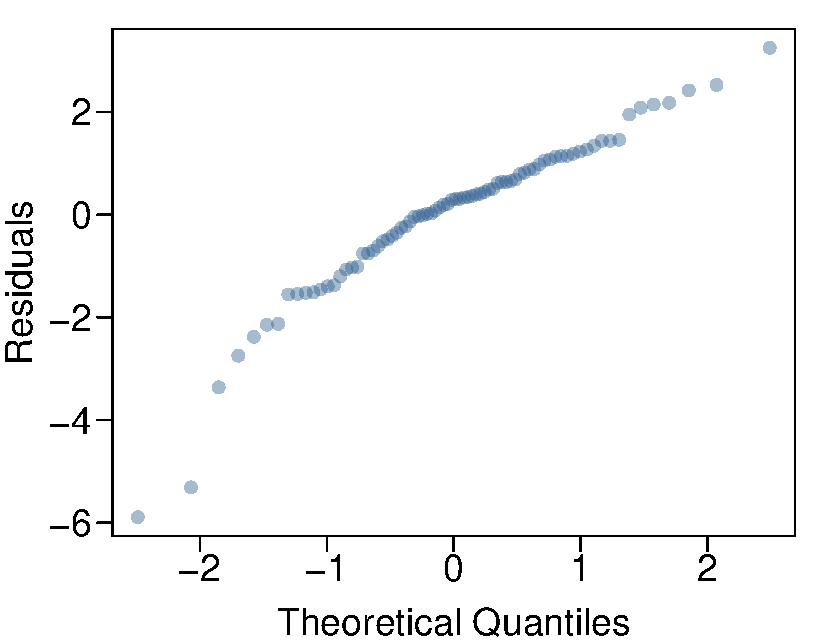
\includegraphics[width=0.325\textwidth]{08/figures/eoce/lmEduNormProbRes} 
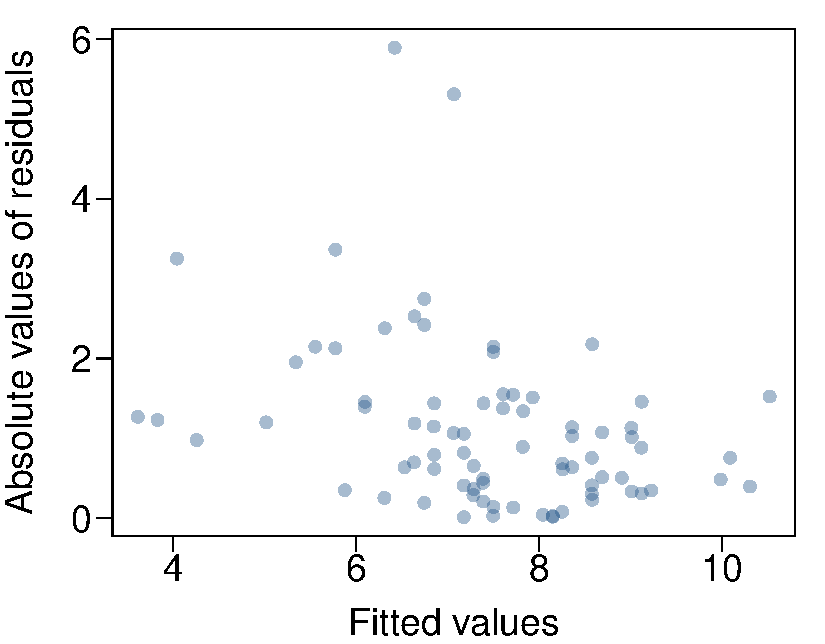
\includegraphics[width=0.325\textwidth]{08/figures/eoce/lmEduAbsResFit} 
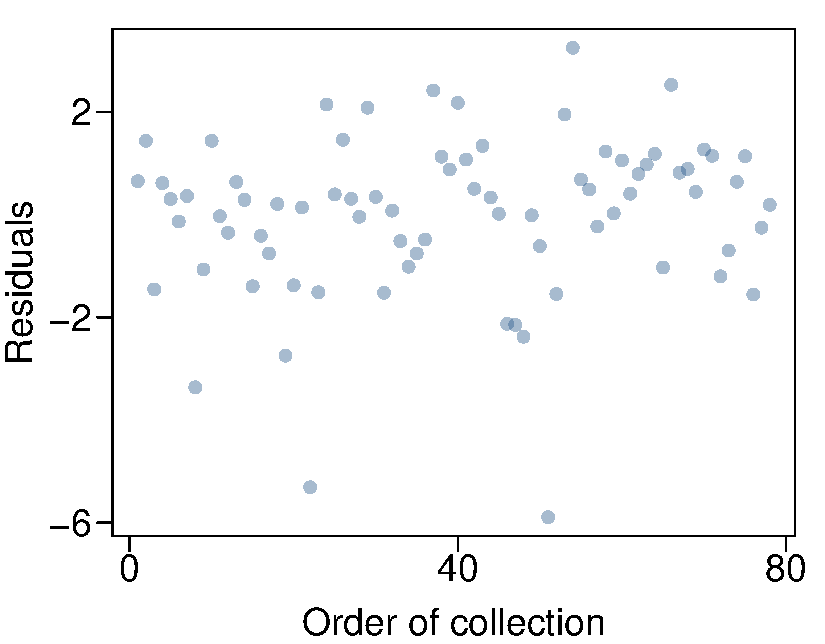
\includegraphics[width=0.325\textwidth]{08/figures/eoce/lmEduResOrder} \\ 
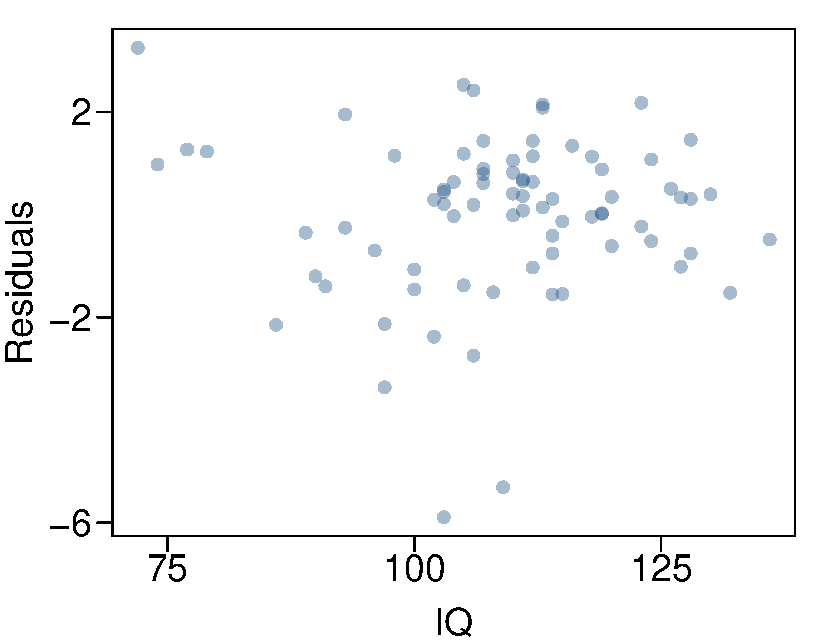
\includegraphics[width=0.325\textwidth]{08/figures/eoce/lmEduResIQ} 
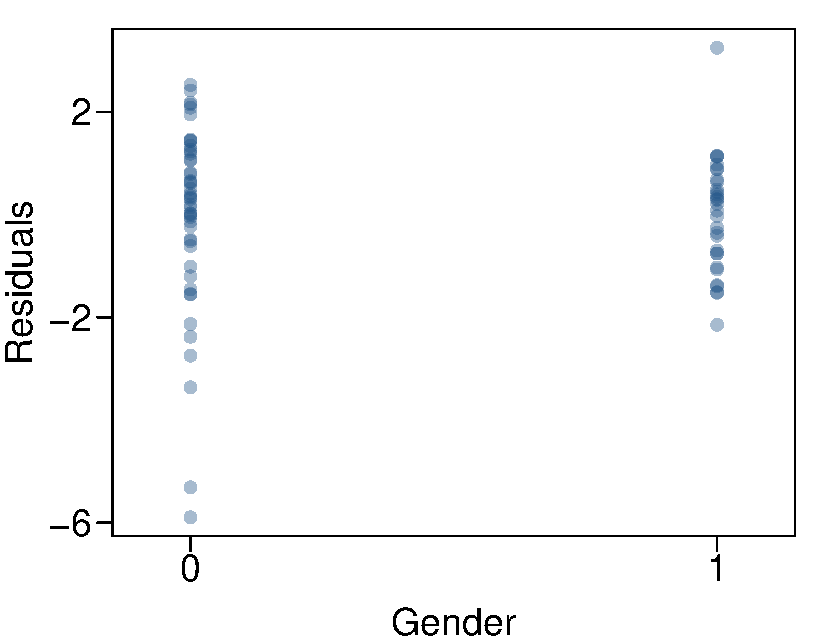
\includegraphics[width=0.325\textwidth]{08/figures/eoce/lmEduResGender} 
\end{center}
}
{
Listed below are four assumptions that should be satisfied for a multiple regression model to be appropriate, and an analysis of whether or not these are met:
\begin{enumerate}[1.]
\item The residuals of the model should be nearly normal: The normal probability plot shows curvature, indicating non-normal residuals.
\item The variability of the residuals should be nearly constant: Couple outliers with high absolute residual values stand out in this plot.
\item The residuals should be independent: While there doesn't seem to be a relationship between the residuals and the order in which the data is collected, this plot reveals couple outliers with large negative residual values.
\item Each variable should be linearly related to the outcome: Residuals vs. IQ and gender plots shows residuals reveals quite a few outliers. There isn't a clear liar relationship between IQ and GPA and the variability of residuals among the two gender groups is not constant.
\end{enumerate}
None of the assumptions are met, most likely due to the outliers in the data. Since the model assumptions are not satisfied we cannot rely on this model to conclude a relationship between the explanatory variables and GPA.
}


%%%%%%%%%%%%%%%%%%%%%

\subsection{ANOVA and regression with categorical variables}

% 15

\eoce{In Exercise~\eoceref{chickwtsCasein}, we considered the effect of casein feed on chicks' weight. Instead of categorizing feed type as casein or other, we might also want to consider all feed types at once: casein, horsebean, linseed, meat meal, soybean, and sunflower. The ANOVA output below can be used to test for differences between the average weights of chicks on different diets.
\begin{center}
\begin{tabular}{lrrrrr}
  \hline
 & Df & Sum Sq & Mean Sq & F value & Pr($>$F) \\ 
  \hline
feed & 5 & 231129.16 & 46225.83 & 15.36 & 0.0000 \\ 
  Residuals & 65 & 195556.02 & 3008.55 &  &  \\ 
   \hline
\end{tabular}
\end{center}
Conduct a hypothesis test to determine if these data provide convincing evidence that the average weight of chicks varies across some (or all) groups. Refer to Exercise~\ref{chickwts} on page~\pageref{chickwts} to assist in checking ANOVA conditions.
}
{
Based on the side-by-side boxplots shown in Exercise~\ref{chickwts}, the constant variance assumption appears to be reasonable. Because the chicks were randomly assigned to their groups (and presumably kept separate from one another), independence of observations is also reasonable. \\
$H_0$: $\mu_1 = \mu_2 = \cdots = \mu_6$ \\
$H_A$: The average weight ($\mu_i$) varies across some (or all) groups. \\
$F_{5,65} = 15.36$ and the p-value is approximately 0. With such a small p-value, we reject $H_0$. The data provide convincing evidence that the average weight of chicks varies across some (or all) groups.
}

% 16

\eoce{A professor who teaches a large introductory statistics class with eight discussion sections would like to test if student performance differs by discussion section. Each discussion section has a different teaching assistant. The summary table below shows the average final exam score for each discussion section as well as the standard deviation of scores and the number of students in each section.
\begin{center}
\begin{tabular}{rrrrrrrrr}
  \hline
 			& Sec 1 & Sec 2 & Sec 3 & Sec 4 & Sec 5 & Sec 6 & Sec 7 & Sec 8 \\ 
  \hline
$n_i$		& 33 & 19 & 10 & 29 & 33 & 10 & 32 & 31 \\ 
$\bar{x}_i$	& 92.94 & 91.11 & 91.80 & 92.45 & 89.30 & 88.30 & 90.12 & 93.35 \\ 
$s_i$ 		& 4.21 & 5.58 & 3.43 & 5.92 & 9.32 & 7.27 & 6.93 & 4.57 \\ 
   \hline
\end{tabular}
\end{center}
The ANOVA output below can be used to test for differences between the average scores from the different discussion sections.
\begin{center}
\begin{tabular}{lrrrrr}
  \hline
 & Df & Sum Sq & Mean Sq & F value & Pr($>$F) \\ 
  \hline
section & 7 & 525.01 & 75.00 & 1.87 & 0.0767 \\ 
  Residuals & 189 & 7584.11 & 40.13 &  &  \\ 
   \hline
\end{tabular}
\end{center}
Conduct a hypothesis test to determine if these data provide convincing evidence that the average score varies across some (or all) groups. Check conditions and describe any assumptions you must make to conduct the test.
}
{
Based on the standard deviations given in the summary table, the constant variance assumption appears to be reasonable. We are not told if the students are randomly assigned to discussion sections, so we cannot be sure of independence of observations. \\
$H_0$: $\mu_1 = \mu_2 = \cdots = \mu_8$ \\
$H_A$: The average score ($\mu_i$) varies across some (or all) groups.
Since the p-value $>$ 0.05, we fail to reject $H_0$. The data do not provide convincing evidence that the average score varies across some (or all) groups.
}

%%%%%%%%%%%%%%%%%%%%%